\chapter{Zeugnis}
\label{zeugnis}
Um Zeugnisse zu Erstellen, m�ssen zuerst die Studierenden in der Liste markiert werden. Danach kann das Zeugnis f�r diese Personen �ber den Men�punkt Dokumente->Zeungis erstellt werden.\\
Es wird immer das Zeugnis des aktuell gew�hlten Studiensemesters erzeugt. Das angezeigte Ausbildungssemester wird dem Status entnommen.\\
\\
\subsection{Noten}
Am Zeugnis werden alle Noten angezeigt, die im Karteireiter Noten eingetragen sind, unabh�ngig davon, ob die Person noch tats�chlich zu dieser Lehrveranstaltung zugeteilt ist.\\
\\
Noten von einzelnen Lehrveranstaltungen k�nnen am Zeugnis ausgeblendet werden. Siehe dazu \ref{lehrveranstaltung}\\
\\
Die Reihenfolge der Lehrveranstaltungen am Zeugnis kann �ber die Lehrveranstaltungsverwaltung ge�ndert werden. Siehe dazu \ref{lehrveranstaltung}\\
\\
\subsection{Projektarbeiten}
Projektarbeiten die im Zuge einer Lehrveranstaltung ausgearbeitet werden, k�nnen am Zeugnis angezeigt werden. Dazu muss die Projektarbeit mit der Lehrveranstaltung verkn�pft sein. Siehe dazu \ref{projektarbeit}\\
\subsection{Auslandsaufenthalt}
Bei Studierenden mit Auslandsaufenthalt, muss im Karteireiter In/Out der Bereich Outgoing (Zeugnis) ausgef�llt werden.\\
Wenn dieser Bereich bef�llt ist, scheint am Zeugnis der Auslandsaufenthalt mit einem entsprechenden Infotext auf.
\subsection{Archivierung}
\begin{figure}
	\centering
	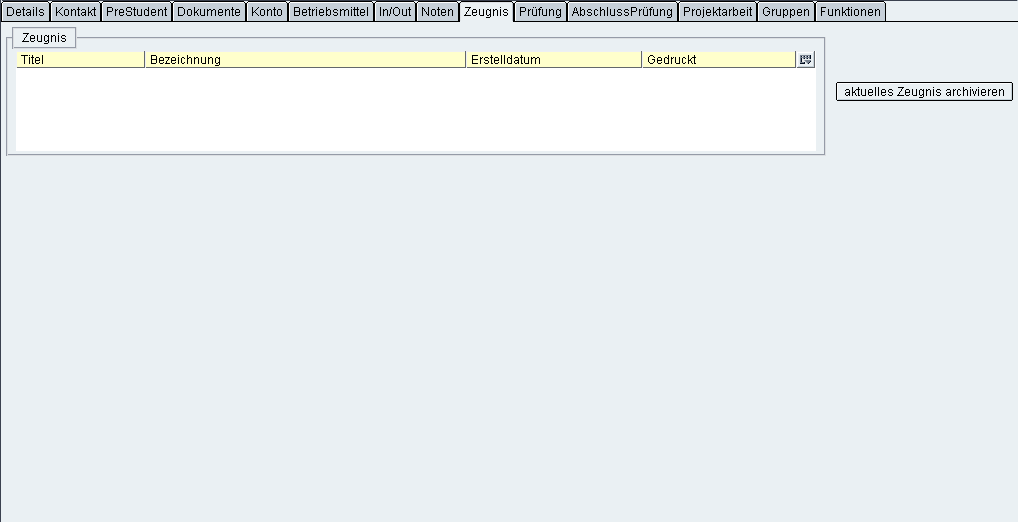
\includegraphics[width=0.75\textwidth]{FAS_Zeugnis1.png}
	\caption{Die Karteikarte Zeugnis}
	\label{zeugnis1}
\end{figure}
Die Karteikarte \textit{Zeugnis}, wie in Abbildung \ref{zeugnis1} gezeigt, hat den Zweck Semesterzeugnisse f�r eine sp�tere Verwendung zu speichern. Dazu wird in das gew�nschte Studiensemester gewechselt und der Student ausgw�hlt. Durch Klicken auf den Button \textit{aktuelles Zeugnis archivieren} wird das Zeugnis des ausgew�hlten Studenten im gew�hlten Studiensemester als Pdf-Datei erzeugt und gespeichtert. Nach Abschlu� des Vorgangs wird das Zeugnis im Listenfeld mit bereits vorhandenen angezeigt. Mit einem Doppelklick wird eine Pdf-Datei ge�ffnet und kann dann gedruckt werden. Ein Rechtsklick bringt die Option das markierte Zeugnis zu l�schen.

Es gibt auch die M�glichkeit die Zeugnisse von mehreren Studenten gleichzeitig zu Archivieren in dem alle Studenten markiert werden und dann auf \textit{aktuelles Zeugnis archivieren} geklickt wird.